\section{液滴的蒸发和燃烧}
\subsection{概述}
\subsection{一些应用}
\subsection{液滴蒸发的简单模型}
\subsubsection{基本假设}
\begin{enumerate}
    \item 液滴在静止、无穷大的介质中蒸发。
    \item 蒸发过程是准稳态的。
    \item 燃料是单成分液体,且其气体溶解度为零。
    \item 液滴内各处温度均匀一致,并假定该温度是燃料的沸点。
    \item 路易斯数为1。
    \item 物性参数为常数。
\end{enumerate}

\subsubsection{气相分析}
这里的分析和第三章的分析是不同的,在这里,蒸发的驱动力是外在的传热,而在第三章中,驱动力主要是扩散。
\begin{enumerate}
    \item 质量守恒;
    \item 能量守恒;
    \item 液-气两相界面能量平衡:
    \[
        \dot{Q}_\text{cond}=\dot{m}(h_\text{vap}-h_\text{liq})=\dot{m}h_\text{fg}
    \]
    这里需要定义个\textit{斯波尔丁数}(\textbf{传递数})\(B\)为:
    \[
        B_q = \frac{c_{pg}(T_\infty-T_\text{boil})}{h_\text{fg}}
    \]
\end{enumerate}

\subsubsection{液滴寿命}

\begin{equation}
    \frac{\dd D^2}{\dd t} = -\frac{8 k_g}{\rho_l c_{pg}}\ln(B_q + 1)
\end{equation}

定义蒸发常数\(K\)为:
\begin{equation}
    K = \frac{8 k_g}{\rho_l c_{pg}}\ln(B_q + 1)
\end{equation}

式子在形式上~\ref{equ:03_evap}是差不多的,如果考虑路易斯数等于1,传热传质效果一样,那就完全一样了。当然,不管路易斯数是不是1,他都是需要满足\(D^2\)定律的:
\begin{equation}
    t_d=D_0^2/K
\end{equation}
这里面需要用到的物性参数近似方法为:
\begin{eqnarray}
    c_{pg} &=& c_{pF}(\overline{T})\\
    k_g &=& 0.4 k_F(\overline{T})+0.6 k_\infty(\overline{T})\\
    \overline{T}&=& (T_\mathrm{boil} + T_\infty)/2
\end{eqnarray}

\subsection{液滴燃烧的简化模型}
\subsubsection{假设}
\begin{enumerate}
    \item 环境精致,液滴之间不互相影响;
    \item 准稳态;
    \item 燃料为单组份,不会互相溶解,液气交界处存在着相平衡;
    \item 压力均匀且为常数;
    \item 气相中只有燃料蒸汽、氧化剂和燃烧产物。气相内部区域只有燃料和产物,外部区域只有氧化剂和产物;
    \item 化学当量比反应,反应无限快,火焰无限薄;
    \item 路易斯数,\(Le=\alpha/\mathcal{D}=k_g/\rho_{c,pg}\mathcal{D}\)为1;
    \item 忽略辐射;
    \item 物性参数都为常数;
    \item 液体燃料液滴是唯一的凝结相,没有碳烟和液体水存在。
\end{enumerate}

\begin{figure}[H]
    \centering
    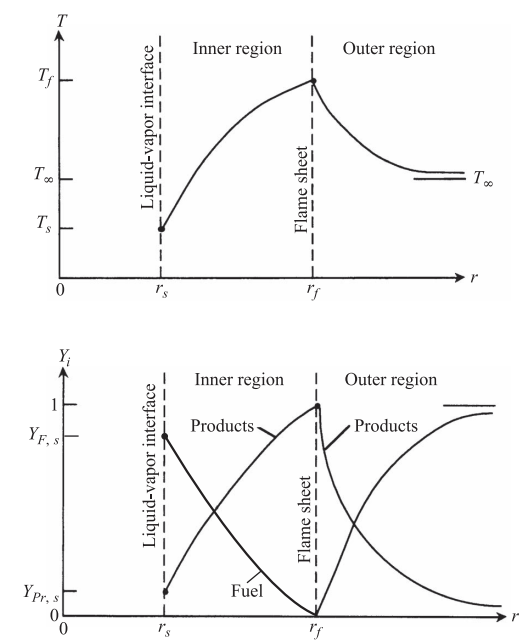
\includegraphics[width=.3\textwidth]{img/drop.png}
\end{figure}

\subsubsection{问题的表述}
求解5个未知数,求解5个关系式:
\begin{enumerate}
    \item 液滴表面的能量平衡
    \item 火焰面处的能量平衡
    \item 外区的氧化剂分布
    \item 内区的燃料蒸汽分布
    \item 液-气界面的相平衡,比如使用克劳修斯-克拉珀龙方程。
\end{enumerate}

\subsubsection{质量守恒}
总流量在任何地方都等于燃料流量.也就是燃烧速率。
\begin{equation}
    {\dot{m}}(r)={\dot{m}}_{F}=\mathrm{constant}.
\end{equation}

\subsubsection{组份守恒}
\textbf{内区}:遵守菲克定律进行扩散。
定义:
\begin{equation}
    Z_F = 1/4\pi\rho\mathcal{D}
\end{equation}

\begin{equation}
    Y_{F,s}=1-\frac{\exp(-Z_{F}\dot{m}_{F}/r_{s})}{\exp(-Z_{F}\dot{m}_{F}/r_{f})}.
\end{equation}

\textbf{外区}:交界处考虑菲克扩散定律的质量通量矢量,如果流入\(\nu\) kg的氧化剂,那么就一定会流出\(\nu+1\)kg的产物,由此我们就可以写出菲克定律,然后根据边界条件,最后解得:
\begin{equation}
    Y_{O x}(r)=\nu\left[{\frac{\exp(-Z_{F}{\dot{m}}_{F}/r)}{\exp(-Z_{F}{\dot{m}}_{F}/r_{f})}}-1\right].
\end{equation}
这里还可以得到燃烧速率和火焰半径之间的关系:

\begin{equation}
    \exp(+Z_F\dot{m}_F/r_f)  = (\nu+1)/\nu
\end{equation}

\subsubsection{能量守恒}
还是用Shvab-Zeldovich形式的能量方程,定义
\begin{equation}
    Z_T = c_{pg}/4\pi k_g
\end{equation}
\begin{enumerate}
    \item 温度分布:代入能量方程直接解酒完事儿了;
    \item 液滴表面能量平衡方程:热是从火焰通过气相导热传到液滴表面的。这些能量一部分用来蒸发燃料,其余的传到液滴内部。
    
    获得向液滴内部导热的集中方法:
    \begin{enumerate}
        \item 将液滴分为两个区,一个处于初始温度区,一个处于表面温度的表面薄层区
        \item 集总参数法;
        \item 忽略液滴的热惯性。
    \end{enumerate}
    \item 火焰面处的热量平衡:火焰处的焓变等于向液滴和无穷远处的能量传递;
    \item 液-气平衡。
\end{enumerate}

如果我们让\(T_f\to T_\infty\)以及\(r_f\to\infty\)那么这就是一个纯纯的蒸发模型,但是由于我们考虑热量传递和质量传递的影响,所以这和前面忽略这两者的简单模型是不同的。

\subsubsection{总结和求解}
定义传递数:
\begin{equation}
    B_{o,q}=\frac{\Delta h_{c}/\nu+c_{p g}\left(T_{\infty}-T_{s}\right)}{q_{i-l}+h_{f g}},
\end{equation}
燃烧速率为:
\begin{equation}
    \dot{m}_{F}=\frac{4\pi k_{g}r_{s}}{c_{p g}}\ln(1+B_{o,q}).
\end{equation}
火焰温度为:
\begin{equation}
    T_{f}=\frac{q_{i-l}+h_{f g}}{c_{p g}(1+\nu)}[{\nu}B_{o,q}-1]+T_{s}
\end{equation}
火焰半径为:
\begin{equation}
    r_{f}=r_{s}\,{\frac{\ln[1+B_{o,q}]}{\ln[(\nu+1)/\nu]}}.
\end{equation}
液滴表面的燃料质量分数为:
\begin{equation}
    Y_{F,s}=\frac{B_{o,q}-1/\nu}{B_{o,q}+1}.
\end{equation}
如果不知道液滴表面的温度,那么我们就需要结合下面的式子进行迭代求解:
\begin{equation}
    T_{s}=\frac{-B}{\ln\!\left[\frac{-Y_{F,s}P M W_{P r}}{A(Y_{F,s}M W_{F}-Y_{F,s}M W_{P r}-M W_{F})}\right]}.
\end{equation}

但是如果认为燃料已经处于沸点了,那么这个时候我们升值连\(Y_{F,s}\)的公式都可以不用,因为那个时候它等于1。

\subsubsection{燃烧速率常数和液滴寿命}

燃烧速率常数\(K\)为:

\begin{equation}
    K = \frac{8 k_g}{\rho_l c_{pg}}\ln(1+B_{o,q})
\end{equation}

在表面温度稳定不变时,这是一个常数。后面就用\(D^2\)定律就好。对于物性参数的选取:
\begin{eqnarray}
    c_{pg} &=& c_{pF} (\overline{T})\\
    k_g &=& 0.4 k_\mathrm{F}(\overline{T}) + 0.6 k_\mathrm{Ox}\\
    \rho_l&=& \rho_l(T_\mathrm{s})\\
    \overline{T} &=& 0.5(T_\mathrm{s}+T_\mathrm{f})
\end{eqnarray}

\textbf{计算差异}:采用上面的方法计算会有下面这些差异
\begin{enumerate}
    \item 实际计算的火焰温度会比一开始估计的火焰温度低好多(因为\(c_\mathrm{pg}\)不合适);
    \item 计算出来的燃烧速率还可以;
    \item 计算出来的无量纲火焰直径比实验值大很多(因为燃料蒸汽积累效应);
    \item 如果我们把环境温度设计成我们估计的火焰温度,按理说在这种纯蒸发的情况下,火焰寿命应该变长,但是实际计算出来却变短了,这是由于“理论”温度低于环境温度,如果我们把算出来的”理论“温度作为环境温度代入,这个时候算出来的纯蒸发的液滴寿命就会比燃烧的液滴寿命要更加长了。
\end{enumerate}

\subsubsection{扩展到对流条件}
\textbf{薄膜理论}的本质是将无穷远处的传热、传质边界条件用所谓的薄膜半径的边界条件替代,且其值相同。
利用\texttt{努赛尔数}\(Nu\)定义传热薄膜半径,\texttt{舍伍德数}\(Sh\)定义传质薄膜半径。
\begin{eqnarray}
    \frac{\delta_\mathrm{T}}{r_s} &=& \frac{Nu}{Nu - 2}\\
    \frac{\delta_\mathrm{M}}{r_s} &=& \frac{Sh}{Sh - 2}
\end{eqnarray}

\begin{eqnarray}
    Nu &=& \frac{h d}{k}\\
    Sh &=& \frac{h d}{\mathcal{D}}
\end{eqnarray}

\begin{figure}[H]
    \centering
    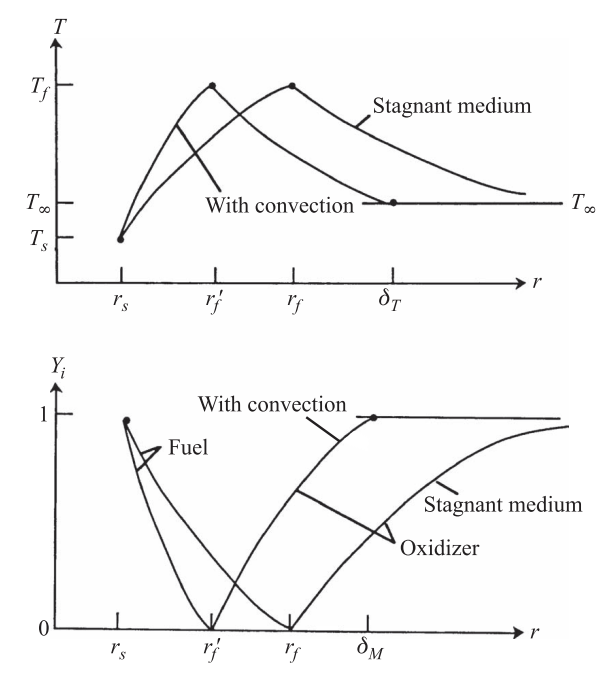
\includegraphics[width=.3\textwidth]{img/convect.png}
\end{figure}
我们相当于借此修改了边界条件的定义:
\begin{eqnarray}
    Y_\mathrm{Ox}(\delta_M) &=& 1\\
    T(\delta_T) &=& T_\infty
\end{eqnarray}

在\(Nu=2\)时,我们认为没有对流出现,在考虑路易斯数=1的情况,传热传质相同,可以得到:

\begin{equation}
    N u=2+\frac{0.557\,R e^{1/2}P r^{1/3}}{[1+1.232/(R e P r^{4/3})]^{1/2}},
\end{equation}
\begin{equation}
    \dot{m}_{F}=\frac{2\pi k_{g}r_{s}N u}{c_{p g}}\ln(1+B_{o,q}),
\end{equation}

\subsection{其他因素}
当环境温度或压力大于蒸发液体的热力学临界点时,只有用变物性才能获得守恒方程的正确表达式。

